\documentclass[utf8x]{beamer}

% \usepackage{beamerthemesplit} // Activate for custom appearance
\usepackage[utf8x]{inputenc}
\usepackage[OT1]{fontenc}
\usepackage{graphicx}
\usepackage{listings}
\usepackage{hyperref}
\usepackage{xcolor}

\usetheme{Malmoe}
\usecolortheme{beaver}

\lstloadlanguages{Python,C,sh}

\definecolor{darkgreen}{RGB}{0,93,21}
\definecolor{greenblue}{RGB}{40,110,126}
\definecolor{lightgray}{RGB}{246,246,246}
\definecolor{bordergray}{RGB}{193,193,193}
\definecolor{lightblue}{RGB}{0,114,168}
\definecolor{methblue}{RGB}{0,31,108}


\title{Extending Theano}
\author{Arnaud Bergeron}
\date{\today}

\lstset{
language=Python,
basicstyle=\fontfamily{pcr}\selectfont\footnotesize,
keywordstyle=\color{darkgreen}\bfseries,
commentstyle=\color{greenblue}\itshape,
stringstyle=\color{violet},
showstringspaces=false,
tabsize=4,
backgroundcolor=\color{lightgray},
frame=single,
%showlines=true,
%emph={theano,MyOp,DoubleOp}, emphstyle=\color{lightblue}\bfseries,
emph={[2]__init__,make_node,perform,infer_shape,c_code,make_thunk,grad,R_op},emphstyle={[2]\color{methblue}},
emph={[3]self},emphstyle={[3]\color{darkgreen}},
moredelim=**[is][{\color{red}}]{`}{`}
}

\newcommand{\code}[1]{\lstinline[emph={[2]}]|#1|}

\begin{document}

\frame[plain]{\titlepage}

\section*{}

\begin{frame}{Outline}
\begin{enumerate}
\item How to Make an Op (Python) (45 min)
\item How to Make an Op (C) (30 min)
\item How to Make a Complex Op (10 min)
\item Optimizations (20 min)
\end{enumerate}
\end{frame}

\section{How to Make an Op (Python)}

\begin{frame}[plain]{}
\begin{center}
\Huge How to Make an Op (Python)
\end{center}
\end{frame}

\begin{frame}[fragile]{Overview}
\lstinputlisting[lastline=14]{python.py}
\end{frame}

\begin{frame}{\code{__init__}}
\lstinputlisting[firstline=6,lastline=8]{python.py}
\begin{itemize}
\item Optional, a lot of Ops don't have one
\item Serves to set up Op-level parameters
\item Should also perform validation on those parameters
\end{itemize}
\end{frame}

\begin{frame}{\code{__props__}}
\lstinputlisting[firstline=4,lastline=5]{python.py}
\begin{itemize}
\item Optional (although very useful)
\item Generates \code{__hash__}, \code{__eq__} and \code{__str__} methods if present
\item Empty tuple signifies no properties that should take part in comparison
\item If you have only one property, make sure you add a final comma: \code{('property',)}
\end{itemize}
\begin{alertblock}{}
Make sure \code{__hash__}, \code{__eq__} and \code{__str__} are not defined in a superclass if you don't inherit directly from Op since otherwise your methods will get shadowed.
\end{alertblock}
\end{frame}

\begin{frame}{\code{make_node}}
\lstinputlisting[firstline=9,lastline=11]{python.py}
\begin{itemize}
\item This creates the node object that represents our computation in the graph
\item The parameters are usually Theano variables, but can be python objects too
\item The return value must be an \code{Apply} instance
\end{itemize}
\end{frame}

\begin{frame}{What Is an Apply Node?}
\begin{center}
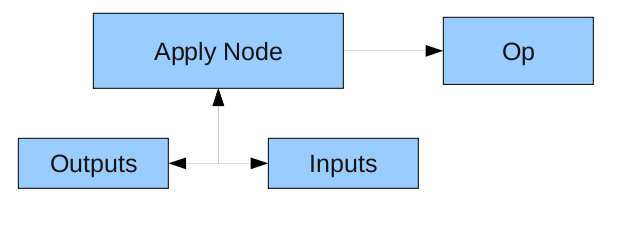
\includegraphics[width=\textwidth]{apply_node}
\end{center}
\end{frame}

\begin{frame}{\code{perform}}
\lstinputlisting[firstline=12,lastline=14]{python.py}
\begin{itemize}
\item This performs the computation on a set of values (hence the method name)
\item The parameters are all python objects (not symbolic values)
\item This method must not return its result, but rather store it in the 1-element lists (or cells) provided in \code{outputs_storage}
\item The output storage may contain a pre-existing value from a previous run that may be reused for storage.
\end{itemize}
\end{frame}

\begin{frame}{DoubleOp}
\lstinputlisting[lastline=15]{doubleop.py}
\end{frame}

\begin{frame}{Op Instances and Nodes}
When you call an op class you get an instance of that Op:
\vskip4mm
\hskip3em\code{double_op = DoubleOp()}
\vskip4mm
But when you want to use that op as a node in a graph you need to call the \textit{instance}:
\vskip4mm
\hskip3em\code{node = double_op(x)}
\vskip4mm
You can do both steps at once with a double call like this:
\vskip4mm
\hskip3em\code{node = DoubleOp()(x)}
\end{frame}

\begin{frame}{Basic Tests}
\lstinputlisting[linerange={1-5,8-18}]{test_doubleop.py}
\end{frame}

\begin{frame}[fragile]{Run Tests}
The simplest way to run your tests is to use \texttt{nosetests} directly on your test file like this:

\begin{lstlisting}[language={},backgroundcolor=\color{white},frame={}]
$ nosetests test_doubleop.py
.
------------------------------------------------------
Ran 1 test in 0.427s

OK
\end{lstlisting}

You can also use \texttt{theano-nose} which is a wrapper around \texttt{nosetests} with some extra options.

\end{frame}

\begin{frame}{Exercise: TripleOp}
What would need to be changed in the code below (DoubleOp) to make this Op triple the input instead of double?
\lstinputlisting[lastline=15]{doubleop.py}
\end{frame}

\begin{frame}{Solution: TripleOp}
You change the class name and the constant \code{2} for a constant \code{3}. \\
\ 
\lstinputlisting[lastline=15]{tripleop.py}
\end{frame}

\begin{frame}{Exercise: ScalMulOp}
\begin{center}
Work though the "06\_scalmulop" directory available at \url{https://github.com/abergeron/ccw_tutorial_theano.git}.
\end{center}
\begin{itemize}
\item Take the \code{DoubleOp} code and make it work with an arbitrary scalar
\item There are more than one solution possible, both have advantages and disadvantages
\end{itemize}
\end{frame}

\begin{frame}{\code{infer_shape}}
\lstinputlisting[firstline=15,lastline=17]{python.py}
\begin{itemize}
\item This functions is optional, although highly recommended
\item It takes as input the symbolic shapes of the input variables
\item \code{input_shapes} is of the form \code{[[i0_shp0, i0_shp1, ...], ...]}
\item It must return a list with the symbolic shape of the output variables
\end{itemize}
\end{frame}

\begin{frame}{Example}
\lstinputlisting[firstline=16,lastline=18]{doubleop.py}
\begin{itemize}
\item Here the code is really simple since we don't change the shape in any way in our Op
\item \code{input_shapes} would be an expression equivalent to \code{[x.shape]}
\end{itemize}
\end{frame}

\begin{frame}{Tests}
To test the \code{infer_shape} method we use \code{InferShapeTester}
\lstinputlisting[linerange={5-5,19-32}]{test_doubleop.py}
\end{frame}

\begin{frame}{Gradient}
\lstinputlisting[firstline=18,lastline=20]{python.py}
\begin{itemize}
\item This function is required for graphs including your op to work with \code{theano.grad()}
\item It must return a list of symbolic graphs for each of your inputs
\item You compute the partial derivative with regards to your inputs
\item Inputs that have no valid gradient should have a special \code{DisconnectedType} value
\end{itemize}
\end{frame}

\begin{frame}{Example}
\lstinputlisting[firstline=19,lastline=21]{doubleop.py}
\begin{itemize}
\item Here since the operation is simple the gradient is simple
\item Note that we return a list
\end{itemize}
\end{frame}

\begin{frame}{Tests}
To test the gradient we use \code{verify_grad}
\lstinputlisting[linerange={5-5,33-41}]{test_doubleop.py}
It will compute the gradient numerically and symbolically (using our \code{grad()} method) and compare the two.
\end{frame}

\begin{frame}{Exercice: Add Special Methods to ScalMulOp}
Work through the "07\_scalmulgrad" directory available at \url{https://github.com/abergeron/ccw_tutorial_theano.git}
\begin{itemize}
\item Take the ScalMulOp class you made and add the \code{infer_shape} and \code{grad} methods to it.
\item Don't forget to make tests for your new class to make sure everything works correctly.
\end{itemize}
\end{frame}

\section{How to Make an Op (C)}

\begin{frame}[plain]{}
\begin{center}
\Huge How to Make an Op (C)
\end{center}
\end{frame}

\begin{frame}{Overview}
\lstinputlisting{c.py}
\end{frame}

\begin{frame}{\code{c_code}}
\lstinputlisting[linerange={9-11}]{c.py}
\begin{itemize}
\item This method returns a python string containing C code
\item \code{input_names} contains the variable names where the inputs are
\item \code{output_names} contains the variable names where to place the outputs
\item \code{sub} contains some code snippets to insert into our code (mostly to indicate failure)
\item The variables in \code{output_names} may contain a reference to a pre-existing value from a previous run that may be reused for storage.
\end{itemize}
\end{frame}

\begin{frame}{Support Code}
\lstinputlisting[linerange={13-14}]{c.py}
\begin{itemize}
\item This method return a python string containing C code
\item The code may be shared with multiple instances of the op
\item It can contain things like helper functions
\end{itemize}
There are a number of similar methods to insert code at various points
\end{frame}

\begin{frame}{Headers, Libraries, Compilers}
Some of the methods available to customize the compilation environment:
\begin{description}
\item[\texttt{c\_libraries}] Return a list of shared libraries the op needs
\item[\texttt{c\_headers}] Return a list of included headers the op needs
\item[\texttt{c\_compiler}] C compiler to use (if not the default)
\end{description}
Again others are available.  Refer to the documentation for a complete list.
\end{frame}

\begin{frame}[allowframebreaks]{Example}
\vskip5mm
This is the C code equivalent to \code{perform}
\vskip4mm
\lstinputlisting[linerange={1-27}]{doublec.py}
\end{frame}

\begin{frame}{COp}
\lstinputlisting{cop.py}
\end{frame}

\begin{frame}{Constructor Arguments}
\begin{itemize}
\item Basically you just pass two arguments to the constructor of COp
\begin{itemize}
\item Either by calling the constructor directly \code{COp.__init__(self, ...)}
\item Or via the superclass \code{super(MyOp, self).__init__(...)}
\end{itemize}
\item The two arguments are:
\begin{itemize}
\item the name of the C code file
\item the name of the function to call to make the computation
\end{itemize}
\end{itemize}
\end{frame}

\begin{frame}{COp: Example}
\only<1>{\lstinputlisting[linerange={1-16}]{doublecop.py}}
\only<2>{\lstinputlisting[language=C]{doublecop.c}}
\end{frame}

\begin{frame}{Tests}
\begin{itemize}
\item Testing ops with C code is done the same way as testing for python ops
\item One thing to watch for is tests for ops which don't have python code
\begin{itemize}
\item You should skip the test in those cases
\item Test for \code{theano.config.gxx == ""}
\end{itemize}
\item Using DebugMode will compare the output of the Python version to the output of the C version and raise an error if they don't match
\end{itemize}
\end{frame}

\begin{frame}{Gradient and Other Concerns}
\begin{itemize}
\item The code for \code{grad()} and \code{infer_shape()} is done the same way as for a python Op
\item In fact you can have the same Op with a python and a C version sharing the \code{grad()} and \code{infer_shape()} code
\begin{itemize}
\item That's how most Ops are implemented
\end{itemize}
\end{itemize}
\end{frame}

\begin{frame}{Exercice: Add C Code to ScalMulOp}
Work through the "08\_scalmulc" directory available at \url{https://github.com/abergeron/ccw_tutorial_theano.git}.
\begin{itemize}
\item Take the ScalMulOp from before and write C code for it using either approach (only accept vectors).
\item You can base yourself on the C code for DoubleOp.
\item Don't forget to test your new implementation! Be sure to check for invalid inputs (matrices).
\end{itemize}
\end{frame}

\section{How to Make a Complex Op}

\begin{frame}[plain]{}
\begin{center}
\Huge How to Make a Complex Op
\end{center}
\end{frame}

\begin{frame}{\code{make_thunk}}
\lstinputlisting[linerange={12-14}]{thunk.py}
\begin{itemize}
\item Define instead of \code{perform} or \code{c_code}
\item Gives total freedom on how the computation is performed
\item More complex to use and generally not needed
\end{itemize}
\end{frame}

\section{Optimizations}

\begin{frame}[plain]{}
\begin{center}
\Huge Optimizations
\end{center}
\end{frame}

\begin{frame}{Purpose}
\begin{itemize}
\item End goal is to make code run faster
\item Sometimes they look after stability or memory usage
\item Most of the time you will make one to insert a new Op you wrote
\end{itemize}
\end{frame}

\begin{frame}{Replace an Op (V1)}
Here is code to use \code{DoubleOp()} instead of \code{ScalMul(2)}.
\lstinputlisting[linerange={1-5,9-15}]{opt.py}
\end{frame}

\begin{frame}{Replace an Op (V2)}
In this case since we are replacing one instance with another there is an easier way.
\lstinputlisting[linerange={1-2,16-20}]{opt.py}
\end{frame}

\begin{frame}{Registering}
In any case you need to register your optimization.
\lstinputlisting[linerange={6-10}]{opt.py}
\lstinputlisting[linerange={21-22}]{opt.py}
\end{frame}

\begin{frame}{Tests}
\lstinputlisting{test_opt.py}
\end{frame}

\begin{frame}{Exercice 4}
Work through the "09\_opt" directory available at \url{https://github.com/abergeron/ccw_tutorial_theano.git}.
\begin{itemize}
\item Make an optimization that replace DoubleOp with DoubleC (or DoubleCOp)
\item Write tests to make sure your optimization is applied correctly
\end{itemize}
\end{frame}

\end{document}
